\documentclass[11pt,a4paper]{article}
\usepackage[top=3cm, bottom=2cm, left=3cm, right=2cm]{geometry}
\usepackage[utf8]{inputenc}
% \usepackage[T1]{fontenc}
\usepackage{amsmath, amsfonts, amssymb}
\usepackage{siunitx}
\usepackage[brazil]{babel}
\usepackage{graphicx}
\usepackage[margin=10pt,font={small, it},labelfont=bf, textfont=it]{caption}
\usepackage[dvipsnames, svgnames]{xcolor}
\DeclareCaptionFont{MediumOrchid}{\color[svgnames]{MediumOrchid}}
\usepackage[pdftex]{hyperref}
\usepackage{natbib}
\bibliographystyle{plainnat}
\bibpunct{[}{]}{,}{s}{}{}
\usepackage{color}
\usepackage{footnote}
\usepackage{setspace}
\usepackage{booktabs}
\usepackage{multirow}
\usepackage{subfigure}
\usepackage{fancyhdr}
\usepackage{leading}
\usepackage{indentfirst}
\usepackage{wrapfig}
\usepackage{mdframed}
\usepackage{etoolbox}
\usepackage[version=4]{mhchem}
\usepackage{enumitem}

\setlist[itemize]{label=\textcolor{CarnationPink}{\textbullet}}

\newcounter{exemplo}

\NewDocumentEnvironment{exemplo}{ O{} }{%
\allowbreak
\setlength{\parindent}{0pt}
  \begin{mdframed}[
  leftline=true,
  topline=false,
  rightline=false,
  bottomline=false,
  linewidth=2pt,
  linecolor=CarnationPink,
  frametitlerule=false,
  frametitlefont=\Large\bfseries\color{CarnationPink},
  frametitle={\color{CarnationPink}\normalfont\bfseries #1},
  ]
}{%
  \end{mdframed}
}

\setlength{\fboxsep}{10pt}
\setlength{\fboxrule}{1pt}
\usepackage{float}
\renewcommand{\thefootnote}{\alph{footnote}}
\usepackage{url}
\hypersetup{
    colorlinks=true,
    linkcolor=cyan,
    filecolor=cyan,      
    urlcolor=cyan,
    citecolor=cyan,
    pdftitle={Proteção Radiológica}
}
\pagestyle{fancy}
\fancyhf{}
\renewcommand{\headrulewidth}{0pt}
\rfoot{Página \thepage}

\title{Resumo}
\author{Notas Rápidas \nocite{*}}
\date{\textit{Dalila Mendonça}}
\begin{document}
	\maketitle


\begin{exemplo}[7. Tratamento com Elétrons]
    \begin{itemize}
        \item Os elétrons perdem sua energia no meio através de interações colisionais (ou seja, ionização e excitação) e interações radiativas (bremsstrahlung). Na terapia com elétrons, as perdas radiativas só se tornam significativas em energias mais altas e materiais de alto Z.
        
        \item A figura abaixo mostra como é a PDP de um feixe de elétrons. As três principais regiões da curva são:
        
            \begin{enumerate}[label=\roman*.]
                \item A região de buildup causada pelo espalhamento lateral dos elétrons que aumenta com o aumento da energia dos elétrons;
                \item A região da queda acentuada de dose, começando em torno da isodose de 90\%; e 
                \item A região da cauda de bremsstrahlung, onde sua magnitude aumenta com o aumento da energia.
            \end{enumerate}
        
            \begin{center}
                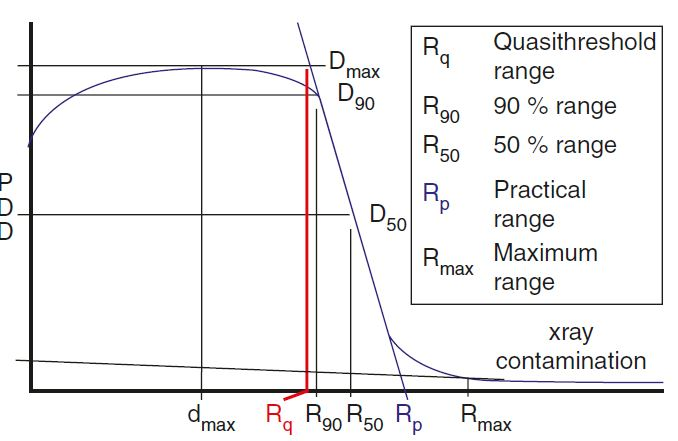
\includegraphics[width=0.5\textwidth]{Imagens/pdpEletrons.JPG}
            \end{center}

        \item O alcance prático ($R_p$) é o parâmetro que determina a profundidade de penetração do elétron. O $R_p$ é definido como o ponto com o qual a tangente da porção descendente da curva de dose na profundidade tem interseção com a curva de extrapolação da cauda de bremsstrahlung. O Alcance prático (em cm) é aproximadamente 1/2 da energia do elétron incidente (em MeV).
        
        \item Ao alterar a SSD em um feixe de elétrons, o comportamento da PDP será praticamente o mesmo, haverá um efeito mínimo na curva da PDP devido a pequena profundidade de penetração do feixe. No entanto, para altas energias de elétrons, o $R_{90}$ (profundidade distal recebendo 90\% da dose, ou seja o alcance de 90\% da dose) será deslocado distalmente alguns milímetros à medida que a SSD aumenta.
        
        \item O $R_{90}$ varia conforme o tamanho de campo. Quando o tamanho de campo está acima de um valor limite, não ocorrerá variação da dose na profundidade. Abaixo desse valor limite, que varia para cada energia de feixe, haverá uma variação significativa da dose na profundidade. Nesses casos, o $R_{90}$ é deslocado cada vez mais em direção à superfície à medida que o tamanho de campo diminui. O $R_p$, por outro lado, é dependente apenas a energia do feixe e portanto não depende do tamanho de campo se mantendo inalterado frente à mudanças do tamanho de campo.
    
        \item Diferentemente dos feixes de fótons, em que a dose na superfície diminui conforme a energia do feixe aumenta, para os feixes de elétrons o aumento da energia faz com que a dose na superfície aumente, de aproximadamente 75\% para 90\% da dose prescrita. O efeito poupador da pele é mínimo para feixes de elétrons e praticamente inexistente em feixes de elétrons de alta energia. 

        \item A colimação dos feixes de elétrons podem ser feitas diretamente na pele ou utilizando um bloco com o recorte da região de tratamento (``cutout''), acoplado ao cone de elétrons. A principal vantagem em utilizar uma colimação diretamente na pele ao invés de utilizar o bloco é que a penumbra é muito mais nítida quando comparado àos cutouts. A colimação na pele é útil para:
        
            \begin{itemize}[label=\textopenbullet]
                \item Tratamentos com campos pequenos;
                \item Fornecer máxima proteção em estruturas críticas adjacentes;
                \item Reduzir a penumbra abaixo do bolus;
                \item Reduzir a penumbra abaixo de um gap de ar extendido ($>$ 5 cm);
                \item Reduzir a penumbra em terapia de elétrons com arco. 
            \end{itemize}
        
        \item A profundidade útil de um feixe de elétrons (em centímetros) é o ponto aproximado onde ocorre as linhas de isodose de 80\% a 90\%, onde $R_{80}(cm) \sim 1/3 E(MeV)$ ou $R_{90}(cm) \sim 1/3.3 E(MeV)$, no entanto $E/4$ também tem sido utilizado para aproximar o $R_{90}$. Porém é importante checar a PDP para um tamanho de campo específico para escolher a energia correta para a profundidade de tratamento necessária. 
        
        \item Existe uma contaminação de raio-x no feixe de elétrons que é resultado da interação de bremsstrahlung dentro do cabeçote do acelerador (que podem acontecer nas folhas espalhadoras, câmaras de ionização, colimadores, etc \dots) e no corpo do paciente. A Contaminação com raios-x aumenta com o aumento da energia, e os valores típicos para a contaminação são:  0.5\% até 1\% para feixes de 6 MeV até 12 MeV; 1\% até 2\% para feixes de 12 MeV até 15 MeV; e 2\% até 5\% para feixes de 15 MeV até 20 MeV.
        
        \item O Bolus é utilizado em tratamentos com eletrons para três finalidades:
        
            \begin{enumerate}[label=\roman*.]
                \item Reduzir as irregularidades da superfície;
                \item Limitar a penetração do feixe de elétrons em certos lugares; e
                \item Aumentar a dose na superfície.
            \end{enumerate}
        O Bolus é feito de um material tecido-equivalente (Z) os materiais mais comuns de bolus são cera, gaze de parafina, superflab e outros plásticos flexíveis.

        \item Caso as PDPs para os campos quadrados $L \times L$ e $W \times W$ sejam conhecidas, a PDP para um campo retangular $L \times W$ em duma determinada profundidade d pode ser determinada a partir da PDP dos campos quadrados através da seguinte relação:
        
            $$PDP(d, L \times W) = \sqrt{PDP(d, L \times L) \cdot PDP(d, W \times W)}$$

        \item Os campos de elétrons são normalmente definidos para que sua incidência seja perpendicular à superfície do paciente. Caso a incidência seja oblíqua à superfície a PDP do feixe de elétrons será modificada, de modo que a incidência oblíqua irá acarretar em:
        
            \begin{enumerate}[label=\roman*.]
                \item um aumento na dose na superfície;
                \item uma dose máxima mais alta;
                \item um deslocamento do $R_{90}$ em direção à superfície; 
            \end{enumerate}

        Estas mudanças são mais significantes em ângulos de obliquidade $>$ \ang{30}.

        \item Ao tratar uma região contendo uma cavidade de ar, a dose na região distal da cavidade nasal é aumentada devido ao maior espalhamento que ocorre em direção a cavidade de ar, enquanto que a dose lateral e distal à  cavidade de ar diminui (ambos os efeitos são devido à perca de equilíbrio lateral). Além disso, o alcance dos elétrons aumenta devido à baixa atenuação nessa região. Portanto, ao tratar regiões que atravessam as cavidades nasais, por exemplo tratamentos de septo nasal, devem ser utilizados tampões nasais para substituir a perda do meio espalhador.
        
        \item Ao tratar uma região que irá atravessar um tecido ósseo, a dose diretamente distal ao osso é diminuída enquanto a dose lateral e distal ao osso é aumentada. Ambos destes efeitos ocorrem devido à perda de equilíbrio de espalhamento lateral. Com o osso, haverá mais espalhamento saindo do osso do que entrando nele o que é oposto ao que ocorre quando o feixe atravessa uma cavidade de ar. 
            
        \item Nos casos de superfícies irregulares com heterogeneidades internas, levarão a uma distribuição de dose complexa com pontos quentes e frios na região de tratamento. Normalmente, para uma protuberância, como o nariz, os pontos quentes estarão em ambos os lados da protuberância e um ponto frio atrás dela; Enquanto que para uma cavidade, como perto do meato acústico externo, a base da cavidade estará quente enquanto seus lados estarão frios. Nesses casos, a utilização de bolus poderá ajudar a aliviar esses efeitos. 
        
        \item Ao utilizar um bolus em um tratamento de elétrons, de forma que o bolus cubra apenas uma parte do campo de tratamento, a borda do bolus irá atuar semelhante a uma protuberância, causando um ponto quente fora do bolus e um ponto frio dentro do bolus. Este efeito pode ser evitado afunilando a borda do bolus. 
        
        \item Ao desenvolver colimações internas para feixes de elétrons, como aquelas utilizadas em Radioterapia Intra-Operatória (IORT) feitas em chumbo, deve-se atentar às seguintes considerações:
        
            \begin{enumerate}[label=\roman*.]
                \item A espessura do colimador deve ser suficiente para parar a radiação; e
                \item O retroespalhamento do elétron pode ser significativo e deve ser considerado no desenvolvimento da colimação, revestindo o colimador com plástico, cera ou cerâmica para blindar os elétrons retroespalhados na blindagem que podem contribuir para um aumento indesejado da dose na região de tratamento. 
            \end{enumerate}

        \item Ao utilizar campos de elétrons adjacentes, forma da isodose na profundidade para os feixes de elétrons levará a formação de pontos quentes e frios na profundidade da adjacência dos campos. Essa heterogeneidade da dose pose ser reduzida, deslocando a borda do feixe em $\pm 1$ cm ao longo do tratamento. 
        
        \item Na IORT, não é possível realizar uma tomografia de planejamento pois o tratamento ocorre no momento da cirurgia. Portanto, o cálculo das MUs necessárias para entrega da dose é feito manualmente, com base em uma profundidade estimada ou determinada no momento da cirurgia, utilizando campos moldados com chumbo ou utilizando aplicadores específicos para a técnica. 
        
        \item Na Terapia em Arco de Elétrons, o gap de ar entre o colimador secundário e o paciente normalmente é maior que o normal, o que irá causar uma maior penumbra. Este efeito pode ser corrigido utilizando uma colimação na pele para deixar a penumbra mais nítida e girar o arco aproximadamente \ang{15} além da borda da área de tratamento.
        
        \item Ao definir a forma da abertura do bloco para tratamento de elétrons, uma possibilidade é desenhar o formato da região de tratamento em um molde em contato com a superfície do paciente. Estima-se que há uma margem de aproximadamente 1 cm entre a borda do alvo e a borda do recorte no bloco quando ambos estão projetados no isocentro. (testar isso aqui!!!)

        \item Conforme a energia do feixe de elétrons aumenta a dose na superfície, a profundidade da isodose de 90\%, o alcance prático e a contaminação com bremsstrahlung também aumenta. A profundidade de dose máxima varia irregularmente com a energia e com o modelo do acelerador.
        
        \item As curvas de isodose de para os feixes de elétrons devem ser determinadas especificamente para cada máquina para as mesmas energias e tamanhos de campo em comum com outras máquinas (não pode-se utilizar os "golden data" para alimentar as pastas de cálculo). Isto se deve ao espalhamento dos elétrons por diferentes componentes físicos presentes no caminho do feixe, que pode mudar de um acelerador para o outro, gerando uma distribuição de dose diferente entre aceleradores apesar de manter as mesmas condições de medida.
        
        \item O retroespalhamento dos elétrons aumenta com o aumento do número atômico e diminui com o aumento da energia do elétron. 
        
        \item Para determinar a dose em um ponto utilizando terapia em arco de elétrons, pode-se medir a dose nesse ponto em um phantom cilíndrico, ou integrar a distribuição de isodose no ponto.
        
        \item Ao utilizar blindagens de feixes de elétrons, diretamente em contato com o pacientes, a dose no tecido em contato com a blindagem irá aumentar pois a blindagem causa o retroespalhamento dos elétrons. Portanto é importante cobrir a proteção com um filtro de número atômico inferior ao da proteção, por exemplo utilizar cera ou plástico nas proteções oculares. É importante lembrar que, o retroespalhamento sempre causará maior dose na região adjacente do material de menor número atômico.
        
        \item A densidade eletrônica relativa de um meio  é determinada em relação a densidade eletrônica da água (meio com o qual o feixe é caracterizado). Por exemplo, a densidade eletrônica relativa para o osso compacto é de 1.6, para o osso esponjoso é de 1.1 e para o pulmão é de 0.2, comparados à densidade eletrônica da agua.

        \item Para determinar a espessura de chumbo necessária para a confecção de um bloco de chumbo utiliza-se a estimativa $T(chumbo)(mm) = 0.5\;mm/MeV$, podendo ser adicionado 1 mm como uma medida de segurança. Normalmente são utilizados blocos feitos de Cerrobend que é aproximadamente 20\% menos denso que o chumbo e portanto, a espessura utilizando o Cerrobend é de 1.2 x T(chumbo). 

        
        \item Diferentemente de um feixe de fótons, que parecem ser originados a partir de um ponto focal (fonte) localizado no alvo de raios-x onde foram produzidos, o feixe de elétrons apresenta um comportamento diferente, de modo que o feixe parece se originar em um ponto virtual no espaço (e não a partir da folha espalhadora), e a posição deste ponto pode mudar dependendo da energia do feixe e do tamanho de campo. Diversas medidas são realizadas à diferentes distâncias que são plotadas em um gráfico para determinar através da extrapolação da curva a posição virtual da fonte, no qual normalmente está logo acima da folha espalhadora. 
        
        \item A posição virtual da fonte é utilizada para calcular a distância da fonte virtual até a superfície ($SSD_{eff}$) afim de estimar o output do feixe com base no inverso quadrado da distância em tratamentos com a SSD estendida. 
        
        \item O feixe estreito de elétrons que sai da guia aceleradora é praticamente monoenergético. No entanto, até chegar ao paciente, o feixe irá interagir com as folhas espalhadoras, colimadores, ar e outras estrutura que estão no seu caminho. Estas interações resultam em uma alargamento do espectro de energia do feixe de modo que a energia média na superfície do paciente é menor que a energia do feixe inicial criado na gia aceleradora.
        
        \item As linhas de alta isodose e baixa isodose se comportam de forma diferente em relação ao tamanho de campo na superfície. As linhas de alta isodose (90\%) são mais estreitas de modo que cobre uma região menor em relação ao tamanho de campo na superfície enquanto que as linhas de baixa isodose são mais largas de modo que cobrem uma região mais larga que o tamanho de campo na superfície. Observando pelo BEV, a isodose de 90\% estaria para dentro da borda do campo e a isodose de 20\% estaria para fora da borda do campo. 
        
        \item Os feixes elétrons são frequentemente utilizados para tratar tumores de pele superficiais, tumores em pequenas profundidades, leitos tumorais e cicatrizes queloidianas. No tratamento de mama, os elétrons podem ser utilizados para tratar a mamária interna, a parede do tórax após a mastectomia (plastrão) e boost (reforço) em leitos tumorais.
        

        \item Ao utilizar um bolus no tratamento com elétrons, o bolus deve ser colocado em contato direto com a  superfície da pele evitando a presença de gaps de ar entre o bolus e pele. A existência de gaps de ar entre o bolus e a pele além de promover um aumento na penumbra do feixe faz com que a dose superficial seja menor que a dose esperada. Isto ocorre devido aos elétrons que são espalhados pelo bolus conseguirem viajar para fora do campo na região do gap de ar, diminuindo a fluência de elétrons que incidem na pele.

    \end{itemize}
\end{exemplo}

\begin{exemplo}[8. Braquiterapia]
    \textcolor{CarnationPink}{Braquiterapia}
    \begin{itemize}
        \item A Braquiterapia é um procedimento especial da Radioterapia que utiliza fontes radioativas colocadas a curtas distâncias do alvo de tratamento. A Braquiterapia fornece distribuições de dose com alto índice de conformidade dentro do volume alvo devido as sementes radioativas (ou fontes) serem colocadas diretamente dentro do alvo ou em suas proximidades.
        
        \item Os tipos de Braquiterapia são:
        
            \begin{itemize}[label=\textopenbullet]
                \item \textcolor{CarnationPink}{\textbf{Braquiterapia Intersticial:}} As fontes radioativas são colocadas diretamente no tecido alvo, ou temporariamente ou permanentemente;
                \item \textcolor{CarnationPink}{\textbf{Braquiterapia Intracavitária:}} As fontes radioativas estão contidas dentro de um aplicador inserido nas cavidades do corpo, como a vagina ou o útero;
                \item \textcolor{CarnationPink}{\textbf{Braquiterapia Intraluminal:}} Se trata de uma subclasse da Braquiterapia Intracavitária, no qual as fontes radioativas são inseridas no lúmen do paciente como os vasos sanguíneos, brônquio, esôfago ou ducto biliar; (\textit{Lúmen é um espaço interno ou cavidade dentro de uma estrutura com formato de tubo num corpo, como as artérias e o intestino})
                \item \textcolor{CarnationPink}{\textbf{Braquiterapia Superficial:}} As fontes radioativas sao colocadas em placas superficiais o moldes que são então colocados na área de tratamento como o olho ou a pele. 
            \end{itemize}

        \item Os sistemas de carregamento das fontes em Braquiterapia são:
        
            \begin{itemize}[label=\textopenbullet]
                \item \textcolor{CarnationPink}{\textbf{Pré-Carregamento Manual:}} Utilizado para sementes de baixa taxa de dose como as utilizadas para tratamento de próstata ou placas oftalmológicas;
                \item \textcolor{CarnationPink}{\textbf{Pós-Carregamento Manual:}}  Atualmente esta técnica não é utilizada com frequência;
                \item \textcolor{CarnationPink}{\textbf{Pós-Carregamento Remoto:}} Técnica utilizada para Braquiterapia de Alta taxa de dose;
            \end{itemize}

        \item O tempo de duração do implante é classificado como:
        
            \begin{itemize}[label=\textopenbullet]
                \item \textcolor{CarnationPink}{\textbf{Implante Permanente:}} As fontes radioativas são permanentemente implantadas dentro do tumor;
                \item \textcolor{CarnationPink}{\textbf{Implante Temporário:}} As fdntes radioativas são implantadas dentro ou perto do tumor e então são removidas uma vez que a dose de radiação prescrita para aquela fração tenha sido entregue.
            \end{itemize}

        \item O ICRU 38 Classifica as faixas de taxa de dose da seguinte forma:
        
            \begin{itemize}[label=\textopenbullet]
                \item \textcolor{CarnationPink}{\textbf{Baixa Taxa de Dose (LDR):}} 0.4 Gy/h - 2.0 Gy/h. Utilizada para implantes permanentes ou pós-carregadores manuais. 
                \item \textcolor{CarnationPink}{\textbf{Média Taxa de Dose (MDR):}} 2Gy/h - 12Gy/h. Pós-carregadores de braquiterapia de taxa de dose pulsada (PDR) foram desenvolvidos neste intervalo de taxa de dose para replicar os efeitos radiobiológicos de um tratamento de LDR em termos da duração total do tratamento, porém emitindo pulsos de radiação com duração variando entre 5 min até 10 min por hora, e não durante todo o tempo de tratamento como ocorre na LDR.
                \item \textcolor{CarnationPink}{\textbf{Alta Taxa de Dose (HDR):}} $>$ 12 Gy/h. A Braquiterapia HDR utiliza uma fonte com alta atividade, normalmente uma fonte de \ce{^{192}Ir} com 10 Ci. O tratamento é entregue utilizando técnicas controladas remotamente. A taxa de dose típica em um tratamento com HDR varia em torno de 100 Gy/h até 300 Gy/h.
            \end{itemize}

        \item Os radionuclídeos mais utilizados em braquiterapia são:
        
            \begin{itemize}[label=\textopenbullet]
                \item Radiação gama de alta energia, como por exemplo: Cs-137, Ir-192 e Co-60;
                \item Radiação gama de baixa energia, como por exemplo: Ir-125 e Pd-103;
                \item Radiação Beta, como por exemplo: P-32, Ru-106, Sr-90 e Y-90;
            \end{itemize}

            Portanto radiação gama e beta são os tipos de radiação mais utilizados em braquiterapia. Muito raramente são utilizados neutrons (Cf-252) e partículas alfa. 


        \item A intensidade da fonte (força da fonte) pode ser especificada em termos da intensidade do Kerma no ar (força Kerma ar - U) para emissores gama; e pode ser especificada em termos de Becquerel (Atividade) (MBq ou GBq) para emissores beta. As unidades Ci e mCi são unidades antigas mas ainda são comumente utilizadas para emissores gama.
        
        \item Os radionuclídeos utilizados em braquiterapia podem estar no estado sólido, líquido e gasoso (como ocorre em fontes de Xe-133). Fontes sólidas são seladas através do encapsulamento em uma camada de metal.
        
        \item As principais vantagens em tratamentos HDR quando comparado a tratamentos LDR são que: $(i)$ O tratamento HDR requer um procedimento ambulatorial, não sendo necessária a internação do paciente; $(ii)$ é um tratamento que requer o uso de afterloaders remotos, levando a uma redução ou eliminação da exposição de radiação da equipe envolvida no processo; $(iii)$ Permite maior controle da distribuição de dose pois a movimentação da fonte permite a otimização da distribuição de dose ajustando o tempo de parada em cada posição de parada para cada canal do afterloader, podendo ser catéter ou agulhas; $(iv)$ É um tratamento com maior estabilidade no posicionamento do aplicador pois leva menos tempo para entregar a dose (menos de uma hora)minimizando a movimentação dos aplicadores durante o tratamento;  $(v)$ A duração mais curta de tratamento permite que seja feito um deslocamento físico de estruturas sadias durante o tratamento, diminuindo a dose recebida no tecido normal; e $(vi)$ devido ao pequeno tamanho das fontes de HDR é possível utilizar aplicadores menores se adequando melhor à estruturas que necessitam de uma cobertura em uma área ou região pequena/estreita.
        

        \item As principais desvantagens em tratamentos HDR quando comparado a tratamentos LDR são que: $(i)$ Um tratamento HDR requer um alto investimento uma vez que os afterloaders possuem alto custo; $(ii)$ Os efeitos radiobiológicos da HDR causam uma maior toxicidade no tecido normal pois a medida que a taxa de dose aumenta, a radiossensibilidade, ou seja, o dano por unidade de dose, aumenta tanto para o tecido tumoral quanto para o tecido normal, porém a radiossensibilidade do tecido normal aumenta mais rapidamente do que a radiossensibilidade do tecido tumoral, aumentando a probabilidade de causar danos ao paciente ao mesmo tempo que o tumor é tratado. Para justificar sua utilização faz-se uso das vantagens de otimização, geometria, estabilidade e redução de dose em tecidos normal além de um esquema de tratamento com múltiplas frações; e $(iii)$ caso o equipamento apresente um mau funcionamento, ou se um paciente estiver em uma situação de emergência, o risco de exposição acidental à radiação é muito maior tanto para o paciente quanto para a equipe no tratamento HDR.
        
        \item Os recursos de segurança e os intertravamentos (interlocks) operacionais necessários para um afterloader HDR são: $(i)$ Sistema Audiovisual; $(ii)$ Monitores de radiação e indicadores de tratamento (luz vermelha indicando que a fonte está exposta); $(iii)$ Interlock de porta;  $(iv)$ Botões de emergência; $(v)$ Manivela de emergência; e $(iv)$ Bateria Reserva (nobreak).
        
        \item 

    \end{itemize}

    \textcolor{CarnationPink}{Braquiterapia LDR}
    \begin{itemize}
        \item 
    \end{itemize}

    \textcolor{CarnationPink}{Braquiterapia HDR}
    \begin{itemize}
        \item 
    \end{itemize}
\end{exemplo}

\begin{exemplo}[9. Técnicas Avançadas de Tratamento]
    \begin{itemize}
        \item 
    \end{itemize}
\end{exemplo}

\begin{exemplo}[10. Tratamentos Especializados]
    \begin{itemize}
        \item 
    \end{itemize}
\end{exemplo}

\begin{exemplo}[11. Qualidade ]
    \begin{itemize}
        \item 
    \end{itemize}
\end{exemplo}


\begin{exemplo}[12. Proteção Radiológica ]
    \begin{itemize}
        \item 
    \end{itemize}
\end{exemplo}

\begin{exemplo}[13. Diagnóstico por Imagem]
    \begin{itemize}
        \item 
    \end{itemize}
\end{exemplo}

\begin{exemplo}[14. IGRT]
    \begin{itemize}
        \item 
    \end{itemize}
\end{exemplo}





\bibliography{ref.bib}
\end{document}